%
% parallelogramm.tex -- Parallelogramm-Regel
%
% (c) 2019 Prof Dr Andreas Müller, Hochschule Rapperswil
%
\documentclass[tikz]{standalone}
\usepackage{amsmath}
\usepackage{times}
\usepackage{txfonts}
\usepackage{pgfplots}
\usepackage{csvsimple}
\usetikzlibrary{arrows,intersections,math}
\begin{document}
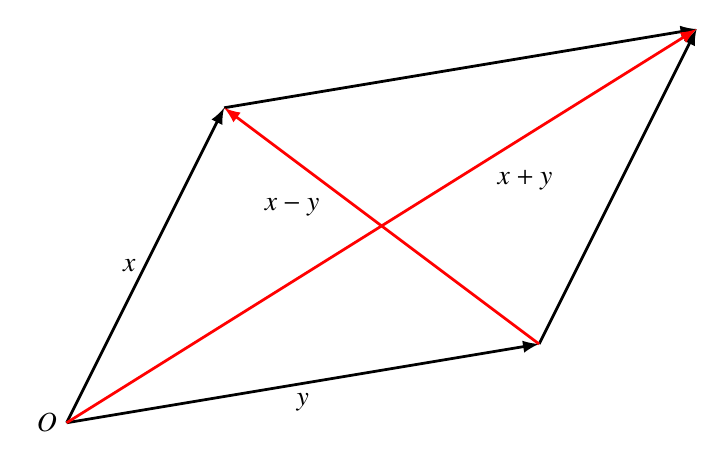
\begin{tikzpicture}[>=latex]

\coordinate (O) at (0,0);
\coordinate (A) at (2,4);
\coordinate (B) at (6,1);
\coordinate (C) at (8,5);

\draw[->,line width=1pt] (O)--(A);
\draw[->,line width=1pt] (A)--(C);
\draw[->,line width=1pt] (O)--(B);
\draw[->,line width=1pt] (B)--(C);

\draw[->,line width=1pt,color=red] (O)--(C);
\draw[->,line width=1pt,color=red] (B)--(A);

\node at (1,2) [left] {$x$};
\node at (3,0.5) [below] {$y$};

\node at (5.333,3.333) [below right] {$x+y$};
\node at (3.333,3) [below left] {$x-y$};

\node at (O) [left] {$O$};

\end{tikzpicture}
\end{document}

